\documentclass{article}

\usepackage{amsmath}
\usepackage{amssymb}
\usepackage{amsthm}
\usepackage{amsfonts}
\usepackage{pgfplots}
\usepgfplotslibrary{fillbetween}
\usepackage[a4paper,margin=0.75in]{geometry}

\title{ST461 Probability - Assignment 3}
\author{Ciarán Ó hAoláín - 17309103 - ciaran.ohaolain.2018@mumail.ie}

\let\nset\varnothing
\let\ddd\cdots

\newtheorem{theorem}{Theorem}[section]
\newtheorem{corollary}{Corollary}[theorem]
\newtheorem{lemma}[theorem]{Lemma}
\theoremstyle{definition}
\newtheorem{definition}{Definition}[section]
\theoremstyle{remark}
\newtheorem*{remark}{Remark}
\theoremstyle{example}
\newtheorem*{example}{Example}

\renewcommand{\d}{\ \mathrm{d}}
\newcommand{\dd}{\mathrm{d}}

\makeatletter
\newcommand{\skipitems}[1]{%
	\addtocounter{\@enumctr}{#1}%
}
\makeatother

%\setlength{\tabcolsep}{20pt}
\renewcommand{\arraystretch}{1.5}

\begin{document}
	\maketitle
	\begin{enumerate}
%		\skipitems{1}
		\item \begin{enumerate}
			\item We have the following (since the joint pmf must sum to 1): \begin{align*}
				k(1+1)+k(1+9)+k(4+9) &= 2k+10k+13k\\
				25k &= 1\\
				k&=\frac{1}{25}
			\end{align*}
			\item We have the table of probabilities:
			\begin{tabular}{ c | c c | c}
				${x \backslash y}$ & 1 & 3 & $\sum$\\
				\hline
				1 & $\frac{2}{25}$ & $\frac{2}{5}$ & $\frac{12}{25}$\\
				2 & - & $\frac{13}{25}$ & $\frac{13}{25}$ \\
				\hline
				$\sum$ & $\frac{2}{25}$ & $\frac{23}{25}$ & -				
			\end{tabular}
			\qquad \qquad  i.e. $\begin{aligned}
				P(X=1)&=\frac{12}{25}\\
				P(X=2)&=\frac{13}{25}\\
				P(Y=1)&=\frac{2}{25}\\
				P(Y=3)&=\frac{23}{25}
			\end{aligned}	$	\\
			This gives us \begin{align*}
				p_X(x)&=
				\begin{cases}
					\frac{12}{25} & x=1\\
					\frac{13}{25} & x=2
				\end{cases}\\
				P_Y(y)&=
				\begin{cases}
					\frac{2}{25} & y=1\\
					\frac{23}{25} & y=3
				\end{cases}
			\end{align*}
			 the marginal probability mass functions of X and Y respectively.
			 \item $P[X>Y]=0,$ as at no point where $P_{XY}$ is non-zero is $x>y$.
		\end{enumerate}
		\skipitems{2}
		\item We can use the following graph:
		\begin{center}
			
			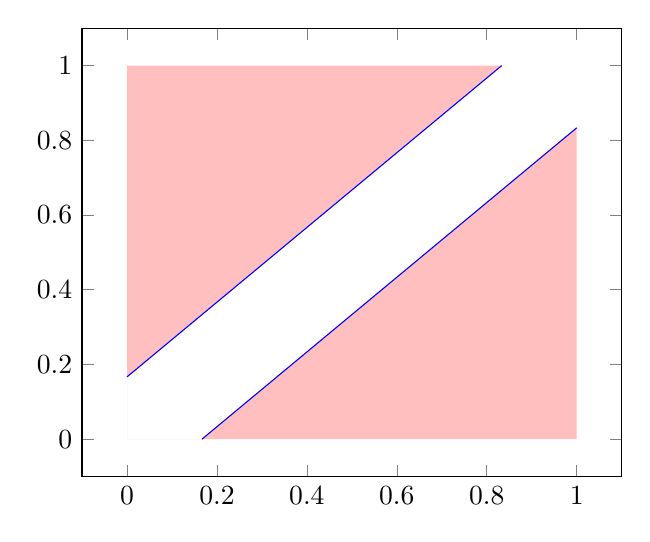
\begin{tikzpicture}
			\begin{axis}[enlargelimits=0.1]
	%		\addplot[name path=f,domain=-0:1,blue] {x};
			\addplot[name path=u,domain=-0:5/6,blue] {x+1/6};
			\addplot[name path=l,domain=1/6:1,blue] {x-1/6};
			
			\path[name path=bottom] (axis cs:0,0) -- (axis cs:1,0);
			\path[name path=top] (axis cs:0,0) -- (axis cs:0,1);
			
			\addplot [
			thick,
			color=blue,
			fill=red, 
			fill opacity=0.25
			]
			fill between[
			of=top and u,
	%		soft clip={domain=0:1},
			];
			\addplot [
			thick,
			color=blue,
			fill=red, 
			fill opacity=0.25
			]
			fill between[
			of=bottom and l,
	%		soft clip={domain=0:1},
			];
			
	%		\node [rotate=48] at (axis cs:  .7,  .59) {$y=x^2$};
	%		\node [rotate=90] at (axis cs:  1.05,  .25) {$x=1$};
			\end{axis}
			
			\end{tikzpicture}
		\end{center}
		
		There is a $\frac{1}{30}=\frac{1}{6}$ of arriving within a given 5 minute range within 30 minutes (uniform distribution).\\
		The non-shaded area, then, is where both people arrive within the same time period.\\
		The red-shaded area is where the people arrive more than five minutes apart.\\
		The two shaded triangles are symmetrical, which means they form a square.\\
		Now we can just find the area of the square.\\
		The square clearly has side length $\frac{5}{6}$ and so we have that the area is $\frac{5}{6}^2=\frac{25}{36}$.\\
		$\therefore$ the probability of the first person waiting more than 5 minutes is $\mathbf{\frac{25}{36}}$.
		
		\item \begin{enumerate}
			\item 
			\begin{align*}
				f_{XY}(x,y)&=f_{X \mid Y}(x \mid y)f_Y(y) & \implies\\
				f_{X \mid Y}(x \mid y)&=\frac{f_{XY}(x,y)}{f_Y(y)}
			\end{align*}
			So we need $f_Y(y)$ which we can find as follows:
			\begin{align*}
				f_Y(y)&=\int_{-\infty}^{\infty}f_{XY} \d x\\
				&=\int_{0}^{1-y}6-6x-6y \d x\
				&=\left[-3x^2-6xy+6x\right]^{1-y}_0\\
				&=-3(1-y)^2-6(1-y)y+6(1-y)\\
				&=-3(1-2y+y^2)+(-6+6y)y+6-6y\\
				&=-3+6y-3y^2-6y+6y^2+6-6y\\
				&=3y^2-6y+3\\
				&=3(y^2-2y+1)
			\end{align*}
			Which means we can find 
			\begin{align*}
				f_{X \mid Y}(x \mid y)&=\frac{f_{XY}(x,y)}{f_Y(y)}\\
				&=\begin{cases}
					2\frac{1-x-y}{y^2-2y+1} & 0 < y < 1-x, x > 0\\
					0 & \mathrm{otherwise}
				\end{cases}
			\end{align*}
			as required.
			\item Since $x,y$ are symmetric in $f_{XY}$ and we've already found $f_Y$, we can deduce that $f_X(x)=f_Y(x)$, i.e. \[f_X(x)=3(x^2-2x+1)\] as required.
			\item $X$ and $Y$ are clearly not independent, since it is clear that \[
			f_{X \mid Y}(x \mid y) \neq f_X(x)\]
			Therefore $X$ and $Y$ are not independent.
		\end{enumerate}

	\end{enumerate}
\end{document}